Model-based methods rely on \emph{planning} as their primary component, while model-free methods
primarily rely on \emph{learning}.


%%%%% SECTION
\section{Models and Planning}
\label{sec:models_and_planning}
\emph{Distribution models}\label{t:distribution_model} produce a description of all possibilities
after a $(s,a)$ pair and their probabilities.
\emph{Sample models}\label{t:sample_model} produce just one of the possibilities after a $(s,a)$
pair, sampled according to the probabilities.
Obviously distribution models are more useful, and if needed they can be used to create samples
and have the output of the sample models.
The opposite is not possible.
The model is used to \emph{simulate} the environment and produce \emph{simulated experience}.
\emph{Planning}\label{t:planning} is a computational process that takes a model as input and
produces or improves a policy for interacting with the modeled environment:
\begin{center}
    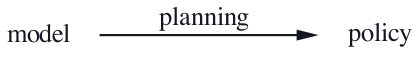
\includegraphics[scale=0.5]{img/model_planning_policy.png}
\end{center}
Two distinct approaches to planning:
\begin{itemize}
    \item \emph{State-space planning}\label{t:state_space_planning}:
        a search through the state space for an optimal policy or an optimal path to a goal.
        Value functions are computed for states or state-action pairs and actions cause
        transitions from state to state.
    \item \emph{Plan-space planning}\label{t:plan_space_planning}:
        a search through the space of plans.
        Operators transform one plan into another, and value functions, if any, are defined over
        the space of plans.
        These methods are difficult to apply efficiently to the stochastic sequential decision
        problems that are the focus in reinforcement learning, and we do not consider them further.
\end{itemize}
All \myref{t:state_space_planning}{state-space planning methods} share a common structure:
\begin{enumerate}
    \item They all involve computing value functions as a key intermediate step to improving the
        policy.
    \item They compute value functions by updates or backup operations applied to simulated
        experience.
\end{enumerate}
\begin{center}
    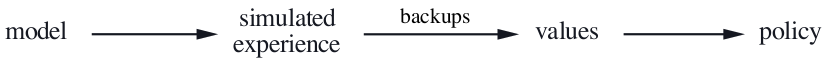
\includegraphics[width=\textwidth]{img/structure_state_space_planning.png}
\end{center}

Planning uses simulated experience generated by a model, learning methods use real experience
generated by the environment.

\begin{center}
    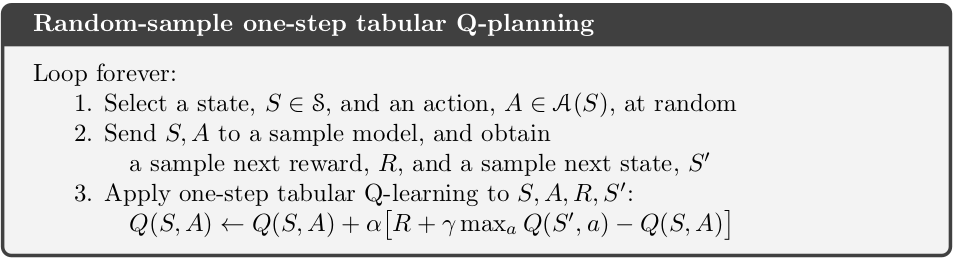
\includegraphics[width=\textwidth]{img/alg_random_sample_one_step_tabular_q_learning.png}
\end{center}


%%%%% SECTION
\section{Dyna: Integrated Planning, Acting, and Learning}
\label{sec:dyna_integrated_planning_acting_and_learning}
\begin{wrapfigure}{r}{0.4\textwidth}
    \centering
    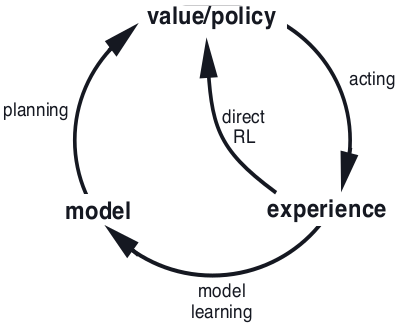
\includegraphics[width=0.4\textwidth]{img/dyna_q_diagram.png}
\end{wrapfigure}
Within a planning agent, there are at least two roles for real experience: it can be
used to improve the model (to make it more accurately match the real environment)
and it can be used to directly improve the value function and policy using the kinds of
reinforcement learning methods we have discussed in previous chapters.
The former we call \emph{model-learning}\label{t:model_learning}, and the latter we call
\emph{direct reinforcement learning} (direct RL).
Dyna-Q includes all of the processes shown in the diagram above - planning, acting,
model-learning, and direct RL - all occurring continually.
\begin{itemize}
    \item planning: one-step tabular Q-planning
    \item direct RL: one-step tabular Q-learning
    \item model learning: stores transitions deterministically in the table
\end{itemize}
During planning the random sampling from the model is done only for $(s,a)$ that have been
experienced.

\begin{figure}[h]
    \centering
    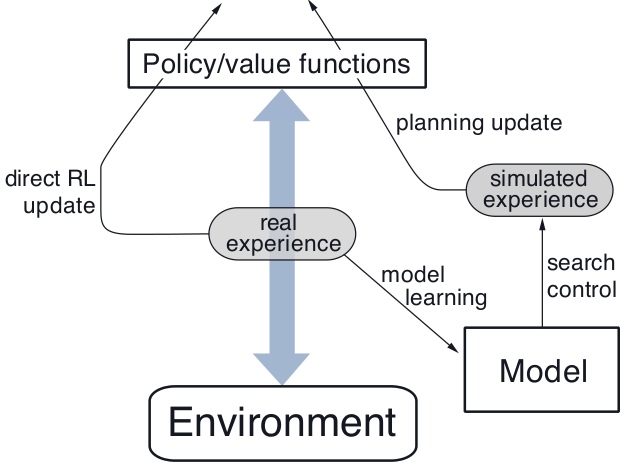
\includegraphics[width=0.8\textwidth]{img/dyna_architecture.png}
    \caption{The general Dyna Architecture.
        Real experience, passing back and forth between the environment and the policy,
        affects policy and value functions in much the same way as does simulated experience
        generated by the model of the environment.}
    \label{fig:dyna_architecture}
\end{figure}

\begin{center}
    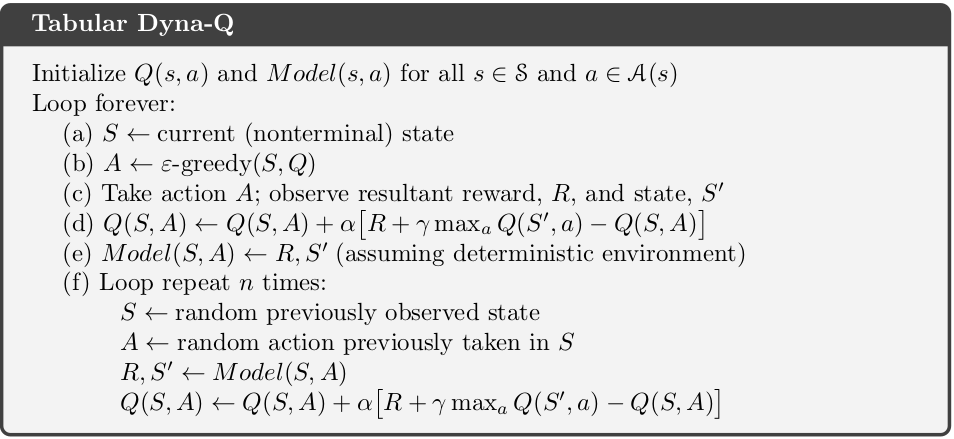
\includegraphics[width=\textwidth]{img/alg_tabular_dyna_q.png}
\end{center}


%%%%% SECTION
\section{When the Model Is Wrong}
\label{sec:when_the_model_is_wrong}
Models may be incorrect because the environment is stochastic and only a limited number of samples
have been observed, or because the model was learned using function approximation that
has generalized imperfectly, or simply because the environment has changed and its new
behavior has not yet been observed.
The suboptimal policy computed by planning quickly leads to the discovery and correction of the
modeling error.
This tends to happen when the model is optimistic in the sense of predicting greater reward or
better state transitions than are actually possible.
The planned policy attempts to exploit these opportunities and in doing so discovers that they do
not exist.

The Dyna-Q+ agent uses a heruistic where it tracks the last time a particular $(s,a)$ pair has
been last tried in a real interaction with the environment.
The more time passes the greater the possibility that the dynamics of the environment under such a
$(s,a)$ pair have changed.
To stimulate the agent to take these exploratory steps a special \emph{bonus reward} is given in
simulated experiences involving these actions.
In particular, if the modeled reward for a transition is $r$, and the transition has not been tried
in $\tau$ time steps, then planning updates are done as if that transition produces a reward
of $r+\kappa\sqrt{\tau}$, for some small $\kappa$.


%%%%% SECTION
\section{Prioritized Sweeping}
\label{sec:prioritized_sweeping}
Pick transitions to learn from using a kind of priority.
Realize that some transitions will not provide any added knowledge, while other might.
It would be good to work \emph{backwards} from goal states, but this notion can be extended to
working back from any state whose value has changed.
One can work backward from arbitrary states that have changed in value, either performing
useful updates or terminating the propagation.
This general idea might be termed backward focusing of planning computations.
A queue is maintained of every state–action pair whose estimated value would change
nontrivially if updated, prioritized by the size of the change.
When the top pair in the queue is updated, the effect on each of its predecessor pairs is
computed.
If the effect is greater than some small threshold, then the pair is inserted in the queue
with the new priority (if there is a previous entry of the pair in the queue, then insertion
results in only the higher priority entry remaining in the queue).
Priority is assigned using \myref{eq:6.8}{td error for Q-learning}.

\begin{center}
    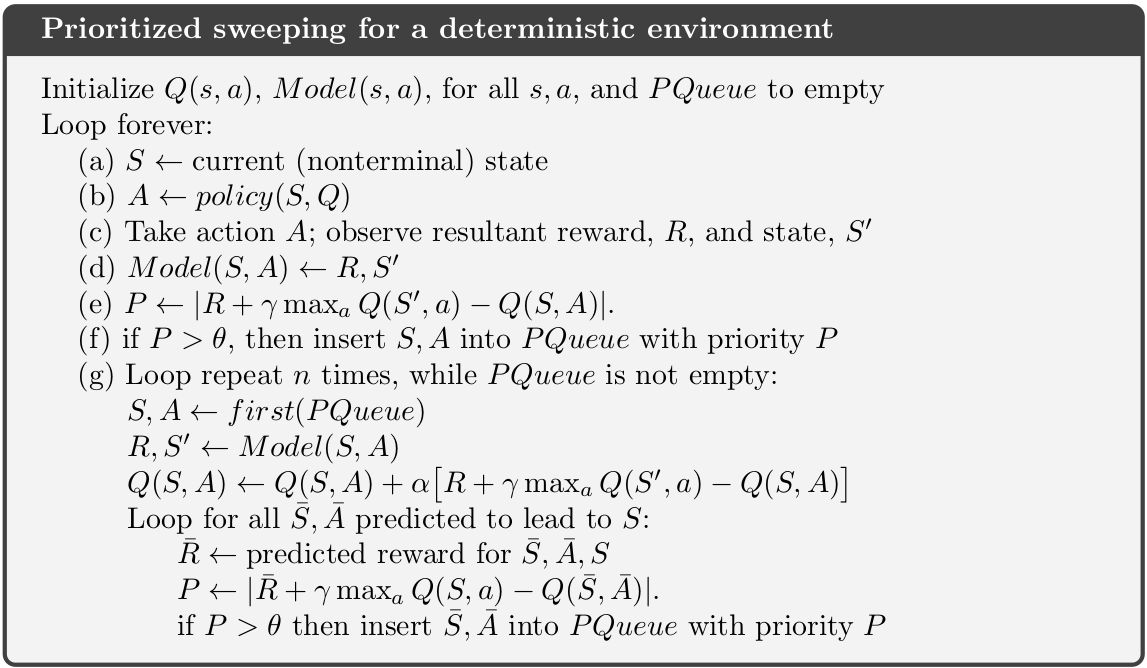
\includegraphics[width=\textwidth]{img/prioritized_sweeping.png}
\end{center}
(g) - backpropagate the update to previous states as long as $\delta$ is over $\theta$.


%%%%% SECTION
\section{Expected vs. Sample Updates}
\label{sc:expected_vs_sample_updates}
